% generated by experiments/make_figures.py from results/primitives.json
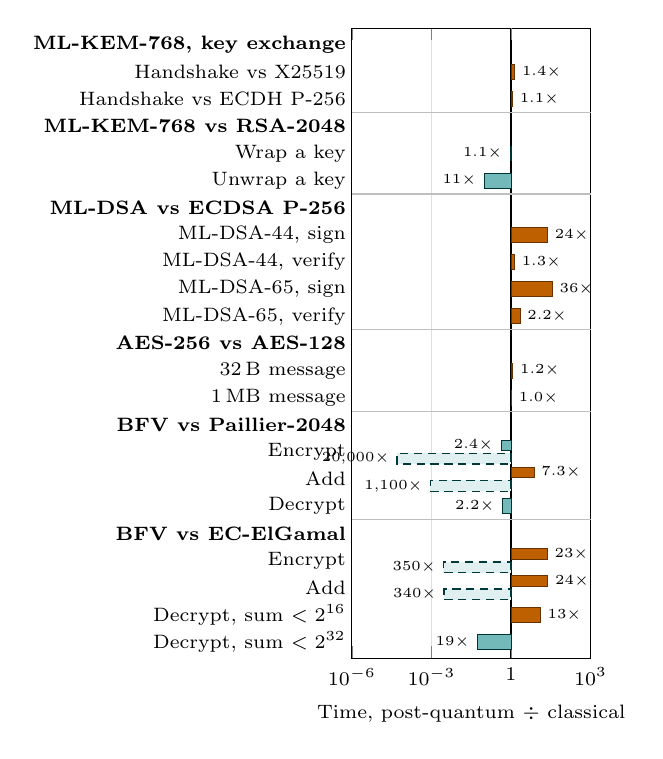
\begin{tikzpicture}[baseline=(current bounding box.north)]
\begin{axis}[
  xmode=log, y dir=reverse, scale only axis,
  width=0.25\textwidth, height=8.0cm, xmin=1e-06, xmax=1000,
  ymin=-0.6, ymax=22.6, ytick={0,...,22}, yticklabels={{\textbf{ML-KEM-768, key exchange}},{Handshake vs X25519},{Handshake vs ECDH P-256},{\textbf{ML-KEM-768 vs RSA-2048}},{Wrap a key},{Unwrap a key},{\textbf{ML-DSA vs ECDSA P-256}},{ML-DSA-44, sign},{ML-DSA-44, verify},{ML-DSA-65, sign},{ML-DSA-65, verify},{\textbf{AES-256 vs AES-128}},{32\,B message},{1\,MB message},{\textbf{BFV vs Paillier-2048}},{Encrypt},{Add},{Decrypt},{\textbf{BFV vs EC-ElGamal}},{Encrypt},{Add},{Decrypt, sum $<2^{16}$},{Decrypt, sum $<2^{32}$}},
  xtick={1e-6,1e-3,1e0,1e3}, xticklabels={$10^{-6}$,$10^{-3}$,1,$10^{3}$},
  tick label style={font=\scriptsize}, label style={font=\scriptsize}, yticklabel style={inner sep=2pt},
  major y tick style={draw=none}, xlabel={Time, post-quantum $\div$ classical}, xmajorgrids, grid style={gray!25}, clip=false,
  extra x ticks={1}, extra x tick labels={}, extra x tick style={grid=major, major grid style={black, line width=0.5pt}},
]
\addplot[draw=none] coordinates {(1,0)};
\filldraw[fill=orange!75!black, draw=orange!40!black, line width=0.2pt] (axis cs:1,0.7245) rectangle (axis cs:1.36088,1.2755);
\node[font=\tiny, anchor=west, inner sep=2.5pt] at (axis cs:1.36088,1.0000) {1.4$\times$};
\filldraw[fill=orange!75!black, draw=orange!40!black, line width=0.2pt] (axis cs:1,1.7245) rectangle (axis cs:1.11893,2.2755);
\node[font=\tiny, anchor=west, inner sep=2.5pt] at (axis cs:1.11893,2.0000) {1.1$\times$};
\draw[gray!50] ({rel axis cs:0,0} |- {axis cs:1,2.5}) -- ({rel axis cs:1,0} |- {axis cs:1,2.5});
\filldraw[fill=teal!55, draw=teal!40!black, line width=0.2pt] (axis cs:1,3.7245) rectangle (axis cs:0.909331,4.2755);
\node[font=\tiny, anchor=east, inner sep=2.5pt] at (axis cs:0.909331,4.0000) {1.1$\times$};
\filldraw[fill=teal!55, draw=teal!40!black, line width=0.2pt] (axis cs:1,4.7245) rectangle (axis cs:0.094307,5.2755);
\node[font=\tiny, anchor=east, inner sep=2.5pt] at (axis cs:0.094307,5.0000) {11$\times$};
\draw[gray!50] ({rel axis cs:0,0} |- {axis cs:1,5.5}) -- ({rel axis cs:1,0} |- {axis cs:1,5.5});
\filldraw[fill=orange!75!black, draw=orange!40!black, line width=0.2pt] (axis cs:1,6.7245) rectangle (axis cs:23.6756,7.2755);
\node[font=\tiny, anchor=west, inner sep=2.5pt] at (axis cs:23.6756,7.0000) {24$\times$};
\filldraw[fill=orange!75!black, draw=orange!40!black, line width=0.2pt] (axis cs:1,7.7245) rectangle (axis cs:1.33173,8.2755);
\node[font=\tiny, anchor=west, inner sep=2.5pt] at (axis cs:1.33173,8.0000) {1.3$\times$};
\filldraw[fill=orange!75!black, draw=orange!40!black, line width=0.2pt] (axis cs:1,8.7245) rectangle (axis cs:35.692,9.2755);
\node[font=\tiny, anchor=west, inner sep=2.5pt] at (axis cs:35.692,9.0000) {36$\times$};
\filldraw[fill=orange!75!black, draw=orange!40!black, line width=0.2pt] (axis cs:1,9.7245) rectangle (axis cs:2.16087,10.2755);
\node[font=\tiny, anchor=west, inner sep=2.5pt] at (axis cs:2.16087,10.0000) {2.2$\times$};
\draw[gray!50] ({rel axis cs:0,0} |- {axis cs:1,10.5}) -- ({rel axis cs:1,0} |- {axis cs:1,10.5});
\filldraw[fill=orange!75!black, draw=orange!40!black, line width=0.2pt] (axis cs:1,11.7245) rectangle (axis cs:1.15634,12.2755);
\node[font=\tiny, anchor=west, inner sep=2.5pt] at (axis cs:1.15634,12.0000) {1.2$\times$};
\filldraw[fill=orange!75!black, draw=orange!40!black, line width=0.2pt] (axis cs:1,12.7245) rectangle (axis cs:1.04195,13.2755);
\node[font=\tiny, anchor=west, inner sep=2.5pt] at (axis cs:1.04195,13.0000) {1.0$\times$};
\draw[gray!50] ({rel axis cs:0,0} |- {axis cs:1,13.5}) -- ({rel axis cs:1,0} |- {axis cs:1,13.5});
\filldraw[fill=teal!55, draw=teal!40!black, line width=0.2pt] (axis cs:1,14.5563) rectangle (axis cs:0.412627,14.9507);
\node[font=\tiny, anchor=east, inner sep=2.5pt] at (axis cs:0.412627,14.7535) {2.4$\times$};
\filldraw[draw=teal!45!black, fill=teal!12, densely dashed, line width=0.45pt] (axis cs:1,15.0493) rectangle (axis cs:5.03695e-05,15.4437);
\node[font=\tiny, anchor=east, inner sep=2.5pt] at (axis cs:5.03695e-05,15.2465) {20{,}000$\times$};
\filldraw[fill=orange!75!black, draw=orange!40!black, line width=0.2pt] (axis cs:1,15.5563) rectangle (axis cs:7.34487,15.9507);
\node[font=\tiny, anchor=west, inner sep=2.5pt] at (axis cs:7.34487,15.7535) {7.3$\times$};
\filldraw[draw=teal!45!black, fill=teal!12, densely dashed, line width=0.45pt] (axis cs:1,16.0493) rectangle (axis cs:0.00089659,16.4437);
\node[font=\tiny, anchor=east, inner sep=2.5pt] at (axis cs:0.00089659,16.2465) {1{,}100$\times$};
\filldraw[fill=teal!55, draw=teal!40!black, line width=0.2pt] (axis cs:1,16.7245) rectangle (axis cs:0.461845,17.2755);
\node[font=\tiny, anchor=east, inner sep=2.5pt] at (axis cs:0.461845,17.0000) {2.2$\times$};
\draw[gray!50] ({rel axis cs:0,0} |- {axis cs:1,17.5}) -- ({rel axis cs:1,0} |- {axis cs:1,17.5});
\filldraw[fill=orange!75!black, draw=orange!40!black, line width=0.2pt] (axis cs:1,18.5563) rectangle (axis cs:23.0802,18.9507);
\node[font=\tiny, anchor=west, inner sep=2.5pt] at (axis cs:23.0802,18.7535) {23$\times$};
\filldraw[draw=teal!45!black, fill=teal!12, densely dashed, line width=0.45pt] (axis cs:1,19.0493) rectangle (axis cs:0.00281741,19.4437);
\node[font=\tiny, anchor=east, inner sep=2.5pt] at (axis cs:0.00281741,19.2465) {350$\times$};
\filldraw[fill=orange!75!black, draw=orange!40!black, line width=0.2pt] (axis cs:1,19.5563) rectangle (axis cs:24.198,19.9507);
\node[font=\tiny, anchor=west, inner sep=2.5pt] at (axis cs:24.198,19.7535) {24$\times$};
\filldraw[draw=teal!45!black, fill=teal!12, densely dashed, line width=0.45pt] (axis cs:1,20.0493) rectangle (axis cs:0.00295385,20.4437);
\node[font=\tiny, anchor=east, inner sep=2.5pt] at (axis cs:0.00295385,20.2465) {340$\times$};
\filldraw[fill=orange!75!black, draw=orange!40!black, line width=0.2pt] (axis cs:1,20.7245) rectangle (axis cs:12.5808,21.2755);
\node[font=\tiny, anchor=west, inner sep=2.5pt] at (axis cs:12.5808,21.0000) {13$\times$};
\filldraw[fill=teal!55, draw=teal!40!black, line width=0.2pt] (axis cs:1,21.7245) rectangle (axis cs:0.0522002,22.2755);
\node[font=\tiny, anchor=east, inner sep=2.5pt] at (axis cs:0.0522002,22.0000) {19$\times$};
\end{axis}
\end{tikzpicture}\hspace{2em}
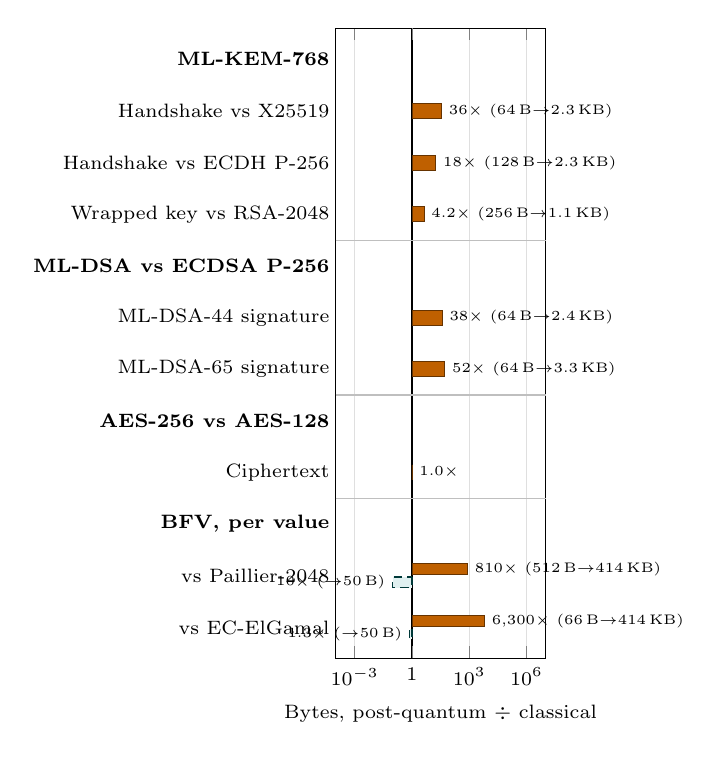
\begin{tikzpicture}[baseline=(current bounding box.north)]
\begin{axis}[
  xmode=log, y dir=reverse, scale only axis,
  width=0.22\textwidth, height=8.0cm, xmin=0.0001, xmax=1e+07,
  ymin=-0.6, ymax=11.6, ytick={0,...,11}, yticklabels={{\textbf{ML-KEM-768}},{Handshake vs X25519},{Handshake vs ECDH P-256},{Wrapped key vs RSA-2048},{\textbf{ML-DSA vs ECDSA P-256}},{ML-DSA-44 signature},{ML-DSA-65 signature},{\textbf{AES-256 vs AES-128}},{Ciphertext},{\textbf{BFV, per value}},{vs Paillier-2048},{vs EC-ElGamal}},
  xtick={1e-3,1e0,1e3,1e6}, xticklabels={$10^{-3}$,1,$10^{3}$,$10^{6}$},
  tick label style={font=\scriptsize}, label style={font=\scriptsize}, yticklabel style={inner sep=2pt},
  major y tick style={draw=none}, xlabel={Bytes, post-quantum $\div$ classical}, xmajorgrids, grid style={gray!25}, clip=false,
  extra x ticks={1}, extra x tick labels={}, extra x tick style={grid=major, major grid style={black, line width=0.5pt}},
]
\addplot[draw=none] coordinates {(1,0)};
\filldraw[fill=orange!75!black, draw=orange!40!black, line width=0.2pt] (axis cs:1,0.8551) rectangle (axis cs:35.5,1.1449);
\node[font=\tiny, anchor=west, inner sep=2.5pt] at (axis cs:35.5,1.0000) {36$\times$ (64\,B$\to$2.3\,KB)};
\filldraw[fill=orange!75!black, draw=orange!40!black, line width=0.2pt] (axis cs:1,1.8551) rectangle (axis cs:17.75,2.1449);
\node[font=\tiny, anchor=west, inner sep=2.5pt] at (axis cs:17.75,2.0000) {18$\times$ (128\,B$\to$2.3\,KB)};
\filldraw[fill=orange!75!black, draw=orange!40!black, line width=0.2pt] (axis cs:1,2.8551) rectangle (axis cs:4.25,3.1449);
\node[font=\tiny, anchor=west, inner sep=2.5pt] at (axis cs:4.25,3.0000) {4.2$\times$ (256\,B$\to$1.1\,KB)};
\draw[gray!50] ({rel axis cs:0,0} |- {axis cs:1,3.5}) -- ({rel axis cs:1,0} |- {axis cs:1,3.5});
\filldraw[fill=orange!75!black, draw=orange!40!black, line width=0.2pt] (axis cs:1,4.8551) rectangle (axis cs:37.8125,5.1449);
\node[font=\tiny, anchor=west, inner sep=2.5pt] at (axis cs:37.8125,5.0000) {38$\times$ (64\,B$\to$2.4\,KB)};
\filldraw[fill=orange!75!black, draw=orange!40!black, line width=0.2pt] (axis cs:1,5.8551) rectangle (axis cs:51.7031,6.1449);
\node[font=\tiny, anchor=west, inner sep=2.5pt] at (axis cs:51.7031,6.0000) {52$\times$ (64\,B$\to$3.3\,KB)};
\draw[gray!50] ({rel axis cs:0,0} |- {axis cs:1,6.5}) -- ({rel axis cs:1,0} |- {axis cs:1,6.5});
\filldraw[fill=orange!75!black, draw=orange!40!black, line width=0.2pt] (axis cs:1,7.8551) rectangle (axis cs:1,8.1449);
\node[font=\tiny, anchor=west, inner sep=2.5pt] at (axis cs:1,8.0000) {1.0$\times$};
\draw[gray!50] ({rel axis cs:0,0} |- {axis cs:1,8.5}) -- ({rel axis cs:1,0} |- {axis cs:1,8.5});
\filldraw[fill=orange!75!black, draw=orange!40!black, line width=0.2pt] (axis cs:1,9.7667) rectangle (axis cs:808,9.9741);
\node[font=\tiny, anchor=west, inner sep=2.5pt] at (axis cs:808,9.8704) {810$\times$ (512\,B$\to$414\,KB)};
\filldraw[draw=teal!45!black, fill=teal!12, densely dashed, line width=0.45pt] (axis cs:1,10.0259) rectangle (axis cs:0.0986328,10.2333);
\node[font=\tiny, anchor=east, inner sep=2.5pt] at (axis cs:0.0986328,10.1296) {10$\times$ ($\to$50\,B)};
\filldraw[fill=orange!75!black, draw=orange!40!black, line width=0.2pt] (axis cs:1,10.7667) rectangle (axis cs:6268.12,10.9741);
\node[font=\tiny, anchor=west, inner sep=2.5pt] at (axis cs:6268.12,10.8704) {6{,}300$\times$ (66\,B$\to$414\,KB)};
\filldraw[draw=teal!45!black, fill=teal!12, densely dashed, line width=0.45pt] (axis cs:1,11.0259) rectangle (axis cs:0.765152,11.2333);
\node[font=\tiny, anchor=east, inner sep=2.5pt] at (axis cs:0.765152,11.1296) {1.3$\times$ ($\to$50\,B)};
\end{axis}
\end{tikzpicture}
